\capitulo{3}{Conceptos teóricos}
En este apartado, se detallan los conceptos teóricos en los que se basa el desarrollo del proyecto, lo que ayudará a los usuarios a comprender mejor su funcionamiento.

\section{API}

Lo primero y más importante que se debe comprender es qué es una API, para que sirve y cuál es su funcionamiento.\cite{api}\\
Una API \textit{'Application Programming Interface'}, o Interfaz de Programación de Aplicaciones es un procedimiento que permite que otra aplicación o software pueda integrar su sistema, permitiendo el uso de sus datos y funcionalidades a través de definiciones y protocolos. \\
El uso de una API sirve para intercambiar información entre servicios a través de una interfaz. Esto facilita su uso, ya que no se requieren conocimientos de implementación del código interno del software a utilizar (Figura 3.1).\\
Las APIs siguen un conjunto de reglas para la comunicación entre los software:
\begin{itemize}
    \item Para empezar, la aplicación del cliente solicita el acceso a la API para recopilar la información que requiere a través de un servidor web ('URI') o identificador uniforme de recursos, el cual se explicará más detalladamente más adelante.
    \item Una vez se ha recibido la solicitud y ha sido validada, se realiza la llamada al programa externo.
    \item El programa externo responde a la API con la información que se ha solicitado.
    \item La API recibe los datos del programa y los transfiere a la aplicación cliente que la ha solicitado inicialmente.
\end{itemize}

\begin{figure}[h!]
    \centering
    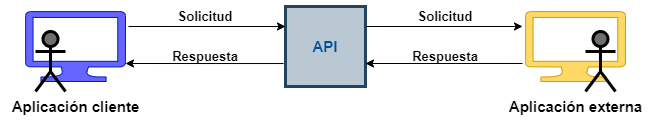
\includegraphics[scale=0.6]{img/APIs.png}
    \caption{Conceptos teóricos - APIs}
    \label{Conceptos teóricos - APIs}
\end{figure}

Podemos encontrar 4 tipos de APIs diferentes:
\begin{enumerate}
    \item APIs públicas: son APIs que pueden ser utilizadas libremente sin tener apenas restricciones.
    \item APIs privadas: son APIs que solo podrán usarse dentro de una propia organización.
    \item APIs de socios: son APIs utilizadas exclusivamente por los socios que competen una alianza comercial.
    \item APIs compuestas: son aquellas que hacen uso de otras APIs de servicio.
\end{enumerate}

\subsection{API de Twitter}

La API de Twitter \cite{apiTwitter} se utiliza para obtener los datos de los tweets según una búsqueda específica, en este caso, Bienes de Interés Cultural del Camino de Santiago Francés en el tramo de Castilla y León (Figura 3.2). \\
\begin{figure}[h!]
    \centering
    
\includegraphics[scale=0.6]{img/APITwitter.png}
    \caption{Conceptos teóricos - API de Twitter}
    \label{Conceptos teóricos - API de Twitter}
\end{figure}

Dependiendo el uso que se le vaya a dar, Twitter ofrece varios niveles de acceso a ella.\\
Desde hace pocas fechas Twitter ha decidido cambiar la política de acceso a su API y los terminos y condiciones que se han utilizado en este proyecto (Figura 3.3).

\begin{enumerate}
    \item {Essential:} es la versión gratuita más básica. Se comenzó utilizando esta, pero más adelante se confirmó que sus recursos no eran suficientes para la realización del proyecto y se debía ascender el nivel de acceso. Permite recopilar 500.000 tweets al mes además de un proyecto por cuenta y acceso a la versión 2 de la API.\\ Sus limitaciones en la hora de la búsqueda son grandes. Lo más importante es que solo permite realizar búsquedas de los tweets más recientes
    
    \item {Elevated:} también es una versión gratuita, pero con más beneficios que la anterior. Permite recopilar 2 millones de tweets al mes y acceso a las versiones 1.1 y 2 de la API de Twitter.
    
    \item {Elevated+:} es un nivel que aún se está desarrollando y no está disponible actualmente. La ventaja que va a tener este nivel es que se podrán realizar hasta 10 millones de búsquedas de tweets al mes.
    
    \item {Academic Research:} este nivel es el utilizado en el proyecto. Para ello, como requisito principal se necesita que se demuestre que eres una persona del ámbito académico mediante un perfil que lo demuestre. No se puede utilizar para el uso comercial, solo para la realización de trabajos o tesis. Aumenta el número de tweets mensuales que pueden buscar a 10 millones y no hay  limitaciones en cuando a fechas de búsqueda, se puede buscar tweets desde la fecha de creación de Twitter.
    
\end{enumerate}
\begin{figure}[h!]
    \centering
    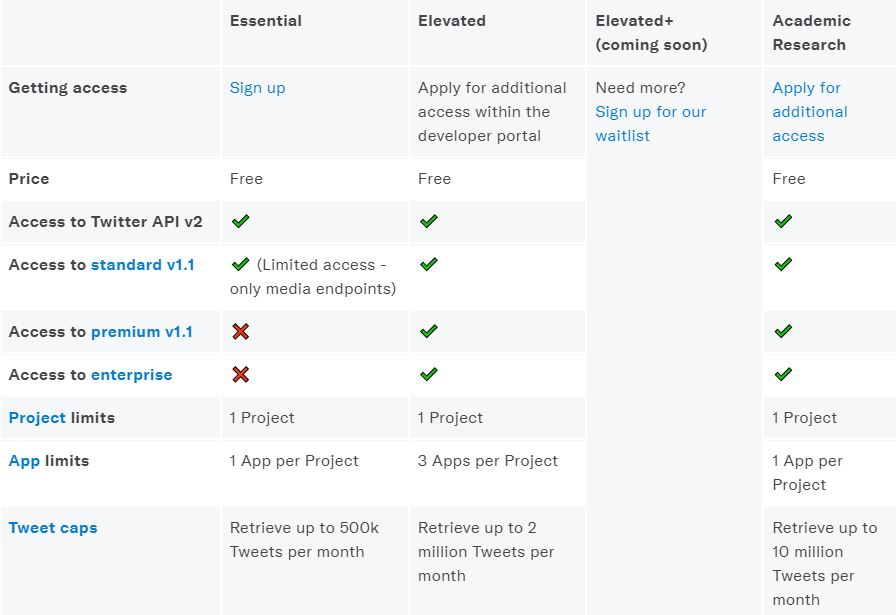
\includegraphics[scale=0.5]{img/nivelesDeAcceso.PNG}
    \caption{Diagrama de secuencia - Niveles de acceso de API Twitter}
    \label{Diagrama de secuencia - Niveles de acceso de API Twitter}
\end{figure}

\subsection{API Endpoint}
El API Endpoint o punto final de la API \cite{apiEndpoint}, es el punto exacto en el que se realiza la comunicación entre la aplicación del cliente y la API. En este punto se dan las solicitudes y respuestas de los implicados, a través de las operaciones GET, POST, DELETE y PATCH.

\subsection{URI}
El identificador uniforme de recursos o \textit{Uniform Resource Identifier} \cite{URI} se utiliza para identificar la información en internet e interactuar con el recurso que la almacena.
La URI está compuesta por cinco partes, dos de ellas obligatorias.
\begin{enumerate}
    \item \textbf{Esquema \textit{('scheme')}}: es una de las partes obligatorias que forman la URI, proporciona información sobre el protocolo que se ha utilizado.
    \item \textbf{Autoridad \textit{('authority')}}: es la parte que identifica el dominio.
    \item \textbf{Ruta \textit{('path')}}: es otra de las partes obligatorias, la cual define la ruta exacta al recurso.
    \item \textbf{Consulta \textit{('query')}}: es la parte define la acción de la consulta.
    \item \textbf{Fragmento \textit{('fragment')}}: se encarga de designar parte del principal recurso.
\end{enumerate}

\section{Series temporales}

Una serie temporal \cite{serieTemporal}es un conjunto de datos ordenados cronológicamente a lo largo de un tiempo determinado. 
Los datos de una serie temporal pueden ser de tres diferentes tipos:
\begin{enumerate}
    \item Datos de series temporales:\\
    Es el más comúnmente utilizado. Se muestran los valores de una variable en diferentes momentos cronológicos.
    \item Datos transversales:\\
    Se muestran en el mismo punto del tiempo los valores de una o más variables.
    \item Datos agrupados:\\
    Es la combinación de mostrar datos de series temporales y datos transversales.
\end{enumerate}
El análisis de las series temporales podemos realizarlo diferenciando cuatro características:
\begin{enumerate}
    \item Tendencia (T):\\
    Movimientos que realiza la serie de manera regular en un largo periodo de tiempo.
    \item Variaciones estacionales (E): \\
    Oscilaciones que realiza la serie temporal a corto plazo de manera regular.
    \item Variaciones cíclicas (C):\\
    Movimientos que realiza la serie temporal a corto plazo, donde el periodo y la amplitud pueden repetirse de manera regular.
    \item Variaciones irregulares o accidentales (A):\\
    Movimientos irregulares que se realizan en las series temporales de manera eventual.
\end{enumerate}
En este proyecto utilizan varios tipos de gráficos para plasmar diferentes tipos de series temporales, los gráficos a mostrar son los siguientes:
\begin{itemize}
    \item Gráfico de líneas:\cite{diagramaLineas}\\
    Es la represención de una o más variables a lo largo del tiempo (Figura 3.4). En este gráfico se podrán detectar repeticiones y si la variable sigue un patrón determinado o por lo contrario se comporta de manera irregular.
    \begin{figure}[h!]
        \centering
        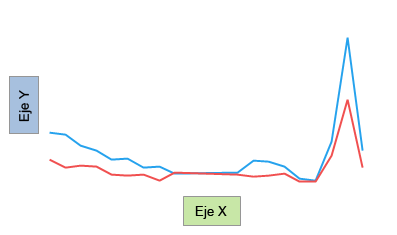
\includegraphics[scale=0.5]{img/GraficoLineas.PNG}
        \caption{Series temporales - Ejemplo de gráfico de lineas}\\
        \label{Series temporales - Ejemplo de gráfico de lineas}
    \end{figure}
    \item Gráfico circular:\cite{diagramaSectores}\\
    Es la manera de representar porcentualmente la frecuencia absoluta de la variable respecto al total durante un periodo de tiempo. \\
    Esta división se realiza sobre una circunferencia, seleccionando el ángulo del porcentaje de la variable a través de la fórmula de la Figura 3.5.
    \begin{figure}[h!]
        \centering
        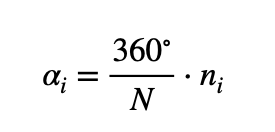
\includegraphics[scale=0.5]{img/FormulaDiagramasSectores.PNG}
        \caption{Series temporales - Fórmula del diagrama de sectores}
        \label{Series temporales - Fórmula del diagrama de sectores}
    \end{figure}
    Un ejemplo visual de cómo sería un gráfico circular se muestra en la Figura 3.6.
    \begin{figure}[h!]
        \centering
        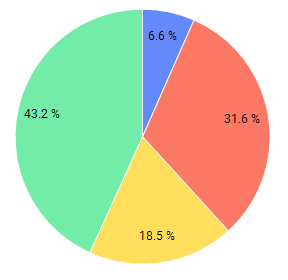
\includegraphics[scale=0.5]{img/GraficoCircular.PNG}
        \caption{Series temporales - Ejemplo de gráfico circular}
        \label{Series temporales - Ejemplo de gráfico circular}
    \end{figure}
    \item Gráfico de barras apiladas:\\
    Es la representación de comparar varias variables en el mismo punto a lo largo del tiempo (Figura 3.7). Estas se representan coloreando cada variable de un color y posicionandolas una encima de otra en el mismo punto en el tiempo hasta que la altura sume el total del valor de las variables en ese momento. Esta operación se repetirá tantas veces como días haya en el periodo de tiempo seleccionado.
    \begin{figure}[h!]
        \centering
        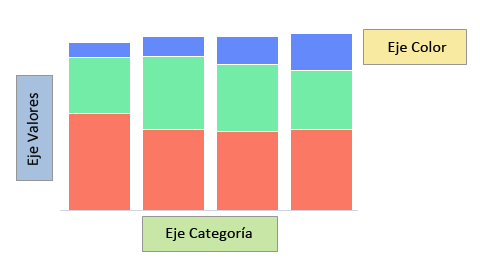
\includegraphics[scale=0.5]{img/GraficoBarrasApiladas.PNG}
        \caption{Series temporales - Ejemplo de gráfico de barras apiladas}
        \label{Series temporales - Ejemplo de gráfico de barras apiladas}
    \end{figure}
\end{itemize}
\section{Aplicación web}
Una aplicación web es un programa o servicio que se ejecuta en internet. Este programa guarda los datos y archivos en ella misma y no necesita que sea desargada en el equipo local.\\
Para realizar el desarrollo web de XacoMeterII se ha utilizado una base de datos, un framework, una plataforma de servicios en la nube y un protocolo HTTP.
\subsection{Base de datos}
Una base de datos \cite{BD} es un contenedor que puede almacenar una gran cantidad de información relacionada y ordenada, que más tarde puede ser buscada de manera mucho más sencilla.\\
Este almacen, además, puede ser manipulado por programas externos a través de unas credenciales.\\
Las bases de datos están formadas por tablas, cada una de ellas con la información que se desee, y además, esas tablas están organizadas por columnas, que son los parámetros diferenciados de la información con un tipo de dato asignado.
Cada uno de los registros de una tabla ordenadas por columnas, se llaman filas.
Las bases de datos se caracterizan por:
\begin{itemize}
    \item \textbf{Redundancia mínima:} la repetición de la información es la mínima, es decir, si un dato ya existe, si se utiliza en la base de datos, no se volverá a repetir.
    \item \textbf{Consistencia de los datos:} al repetir el menor número de información posible, se consigue que las actualizaciones o los borrados se realicen completamente, es decir, que todas las copias de la información sean consistentes.
    \item \textbf{Acceso concurrente por parte de múltiples usuarios:} el uso de una base de datos permite el acceso de varios usuarios al mismo tiempo, pudiendo mostrar toda la información necesaria simultáneamente.
    \item \textbf{Integridad de los datos:} una base de datos asegura poder recuperar los datos sin importar su antigüedad.
    \item \textbf{Consultas complejas optimizadas:} como la información de la base de datos está ordenada y organizada por parámetros, se puede buscar fácilmente y más rápido la información más compleja de encontrar.
    \item \textbf{Acceso a través de lenguajes de programación:} una base de datos permite acceder a ella a través de programas externos con varios lenguajes de programación.
\end{itemize}   
En este proyecto se utiliza una base de datos con lenguaje SQL \cite{sql}, que permite trabajar con los datos y las relaciones de los mismos.
Este lenguaje SQL permite las siguientes operaciones en una base de datos:
\begin{enumerate}
    \item \textbf{MOSTRAR:} a través de la operación 'SELECT'.
    \item \textbf{ACTUALIZAR:} a través de la operación 'UPDATE'.
    \item \textbf{INSERTAR:}  a través de la operación 'INSERT'.
    \item \textbf{BORRAR:} a través de la operación 'DELETE'.
\end{enumerate}
\subsection{Framework}
Un \textit{framework} \cite{framework} es una estructura base que sirve para el desarrollo de aplicaciones reutilizando herramientas y módulos. 
A través de los \textit{framework} se consigue reducir el tiempo de programación y los errores causados.
Dependiendo del lenguaje de programación se podrá elegir entre varios \textit{framework}. En este caso, XacoMeterII es un proyecto desarrollado en Python, por lo que se ha considerado que lo más conveniente es utilizar el \textit{framework} 'Flask'.

\subsection{Plataforma de servicios en la nube}
Una plataforma como servicio (PaaS) \cite{PaaS} es un conjunto de servicios integrados en la nube que permiten a los desarrolladores incluir todo lo necesario  para crear, ejecutar y gestionar aplicaciones.\\
En este proyecto se utilizará una plataforma de servicios en la nube (PaaS) llamada Heroku que permitirá el despliegue de la aplicación en la nube para que pueda ser utilizada por todos los usuarios de internet (Figura 3.8).
\begin{figure}[h!]
    \centering
    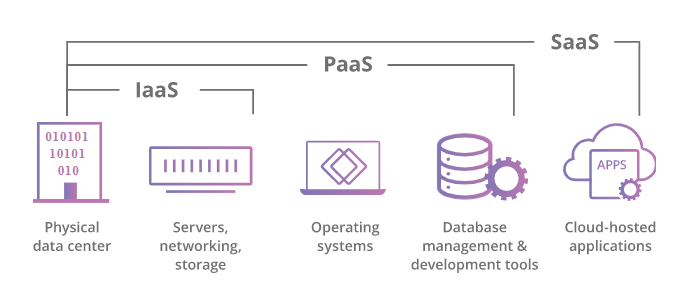
\includegraphics[scale=0.6]{img/PaaS.PNG}
    \caption{Conceptos teóricos - Plataforma de servicios en la nube}
    \label{Conceptos teóricos - Plataforma de servicios en la nube}
\end{figure}

\subsection{Protocolo HTTP}
El protocolo HTTP \textit{(Hypertext Transfer Protocol)} \cite{HTTP} es la manera que tienen de comunicarse un cliente con un servidor. El cliente solicita la información y el servidor se lo devuelve a modo de respuesta.
HTTP es un protocolo que no tiene estado: el cliente realiza una petición al servidor, este contesta y la transacción acaba, con lo que en la siguiente petición que pueda realizar el mismo cliente se deben proporcionar de nuevo todos los datos necesarios para que el servidor sirva correctamente la nueva petición.
\subsection{Sentiment analysis}
El proceso de Análisis de Sentimiento \cite{analisisSentimientos} consiste en la evaluación computacional de emociones, actitudes y opiniones presentes en un texto dado. Esta técnica es ampliamente utilizada por organizaciones para obtener la reacción de los clientes en relación a un producto o servicio en particular.\\
El Análisis de Sentimiento se realiza mediante el uso de tecnologías avanzadas de Inteligencia Artificial, incluyendo el Procesamiento del Lenguaje Natural, el Análisis de Texto y la Ciencia de Datos, con el objetivo de identificar, extraer y analizar información subjetiva presente en un texto. La herramienta clasifica un texto en tres categorías principales: positivo, negativo o neutral. 
\\En este caso específico, se utiliza una librería \cite{SentimentAnalysisSpanish} basada en Redes Neuronales para predecir el sentimiento de frases en español.\\
Sentiment-Analysis-Soanish ha entrenado una red neuronal convolucional con datos extraídos de diferentes páginas webs y redes sociales.
